\documentclass[laporan.tex]{subfiles}

\begin{document}

\chapter{METODE PENELITIAN}

\section{Metode Penelitian}

Dalam bab ini akan diuraikan mengenai metode yang digunakan dalam penelitian. Metode penelitian menurut Sugiyono pada dasarnya merupakan cara ilmiah untuk mendapatkan data dengan tujuan dan kegunaan tertentu.

Penelitian yang penulis lakukan adalah penelitian analisis. Penelitian analisis adalah penelitian yang dimulai dari teori dan berakhir dengan fakta , karenanya dalam riset ini ada lebih dari satu hipotesisi yang terlibat. Teori berfungsi sebagai masukan sekaligus sebagai pemecahan masalah yang bersangkutan

\section{Objek Penelitian}

Objek penelitian yang penulis gunakan dalam penelitian ini adalah jeruk keprok (\emph{Citrus sinenesis}). Fokus pengamatan adalah cacat pada tekstur kulit jeruk.

\section{Jenis dan Sumber Data}

Pada penelitian ini, penulis menggunakan beberapa jenis data.

\subsection{Data Primer}

Data primer adalah data yang diperoleh secara langsung, dapat diperoleh melalui wawancara atau observasi secara langsung. Data yang penulis gunakan adalah berupa foto-foto jeruk keprok dari berbagai kelas kualitas.

\subsection{Data Sekunder}

Data sekunder adalah data primer yang sudah diolah lebih lanjut dan disajikan dengan baik oleh pihak pengumpul data primer atau pihak lainnya. Data yang penulis gunakan diolah dari foto-foto jeruk yang telah dipersiapkan

Selain itu, penulis juga mengumpulkan data melalui studi literatur, yaitu dengan mempelajari jurnal dan hasil penelitian yang sudah ada untuk mendapatkan pemahaman tentang analisis tekstur.

\section{Analisis Kebutuhan Perangkat}

Tujuan  dari  proses analisa kebutuhan aplikasi adalah untuk mengetahui sifat dari  kebutuhan  sistem  sehingga  mempermudah  dalam perancangan. Tujuan lain dari analisa ini adalah untuk mendokumentasikan sifat  program  tersebut. Proses analisis meliputi analisis kebutuhan perangkat lunak dan perangkat keras, termasuk analisis terhadap kebutuhan sistem.

\subsection{Kebutuhan Perangkat Lunak}

\begin{description}

\item [Octave] 
\emph{Software} yang digunakan dalam penelitian ini adalah Octave dengan \emph{package} \texttt{image} untuk melakukan pemrosesan citra dan pengolahan data secara numerik. Matlab dapat digunakan sebagai pengganti Octave.

\end{description}

\subsection{Kebutuhan Perangkat Keras}

\begin{enumerate}

\item PC yang dapat menjalankan perangkat lunak Octave
\item Kamera minimum 2MP
\item Lampu LED 5W
\item Backdrop kain hitam

\end{enumerate}

\subsection{Tahapan Penelitian}

Langkah-langkah penelitian yang harus dilakukan yaitu:

\begin{enumerate}
\item mengambil foto-foto jeruk dari berbagai kualitas, Untuk akurasi data maka pengambilan foto perlu dilakukan pada kondisi yang terkontrol.
\item pengolahan awal foto
\item perhitungan \emph{threshold} komponen warna
\item klasifikasi \emph{pixel} awal
\item perhitungan rata-rata intensitas setiap kelas
\item pembuatan kelas baru
\item klasifikasi \emph{pixel} akhir
\item pembuatan \emph{mask} untuk menandai objek jeruk dan daerah-daerah cacat pada jeruk
\item perhitungan luas daerah cacat pada permukaan kulit jeruk
\item perhitungan akurasi hasil deteksi
\end{enumerate}

\subsubsection{Pengambilan Foto} \label{photoshoot}

Pengambilan foto dilakukan dengan perlengkapan-perlengkapan berikut

\begin{enumerate}
\item Kamera DSLR Nikon D3100
\item Sumber cahaya lampu LED Philips 5W dan \emph{stand}
\item Kain hitam
\end{enumerate}

Kamera DSLR diset sebagai berikut: 
\begin{enumerate}
\item sensitivitas ISO 200
\item mode pencahayaan \emph{aperture priority}
\item format citra JPEG dengan resolusi 3406x2304 \emph{pixel}
\end{enumerate}

Kamera, sumber cahaya dan objek disusun sebagai Gambar \ref{fig:setup}. Jarak antara kamera dan objek adalah 50cm.
% 50cm
\begin{figure}[h]
\centering
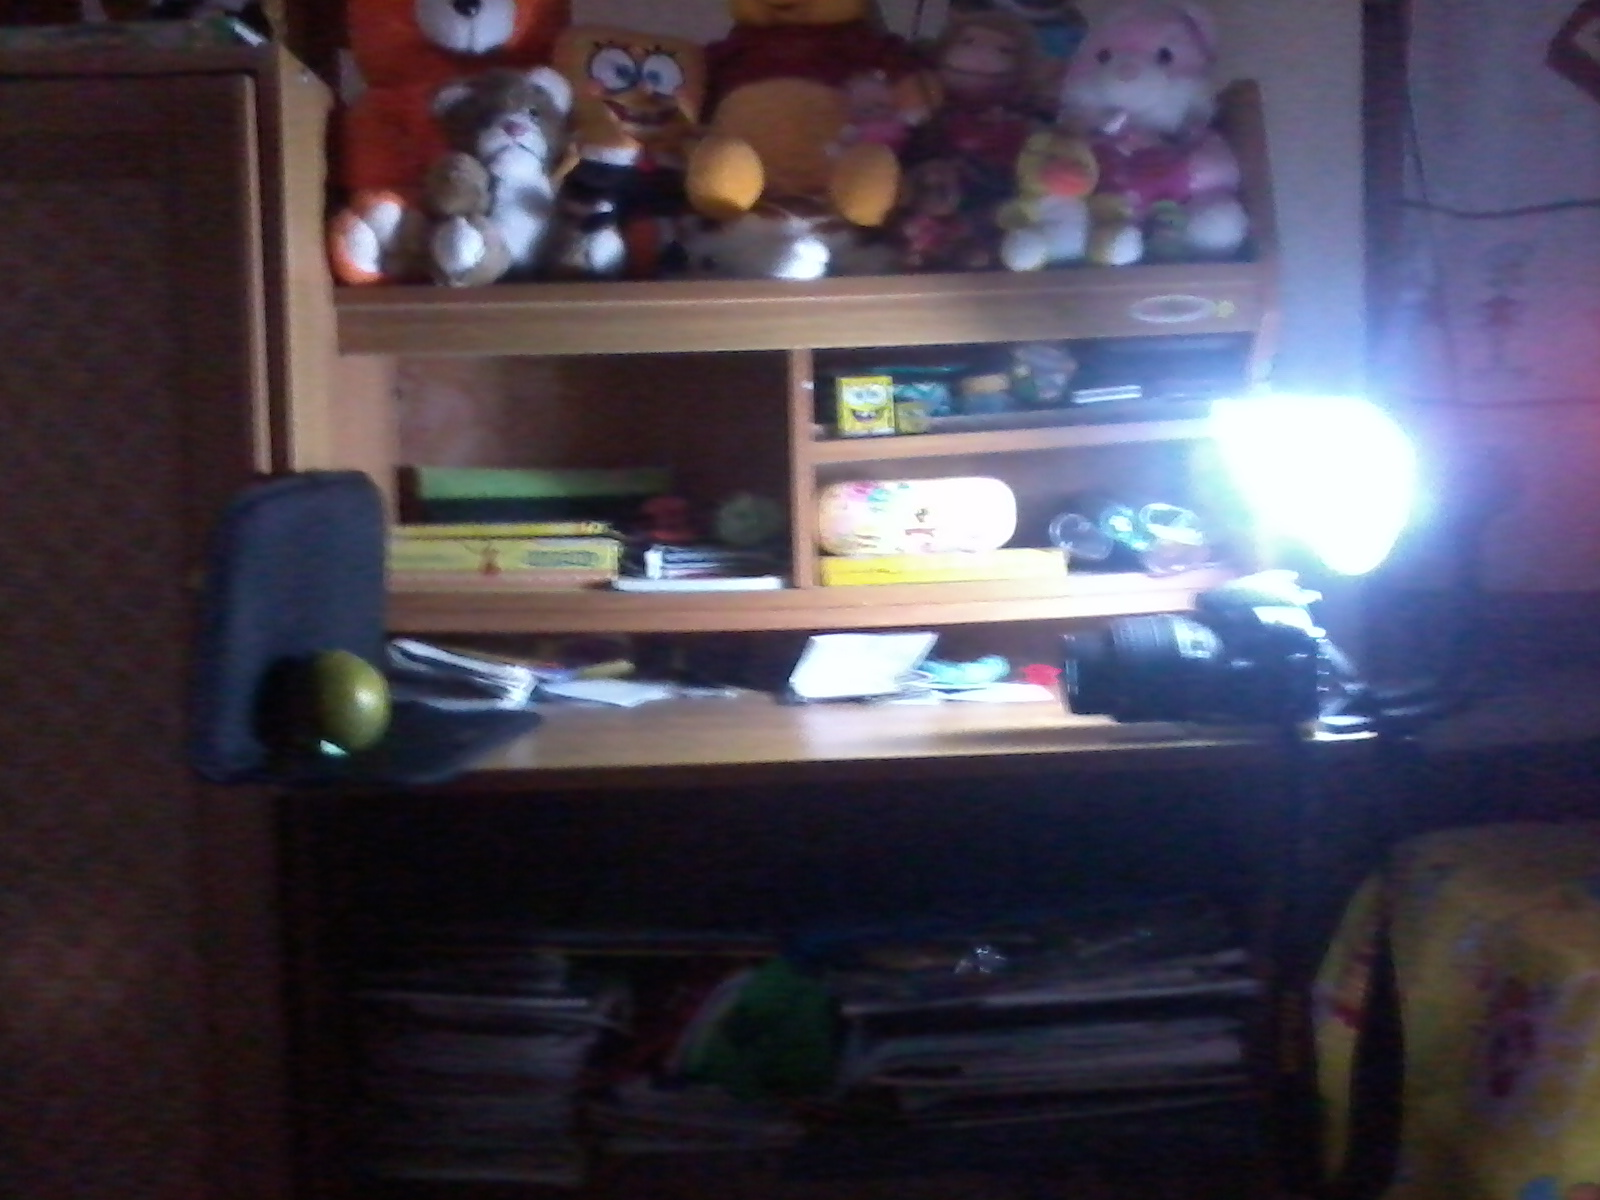
\includegraphics[width=8cm]{tex/Photo-0776.jpg}
\caption{Penataan kamera, sumber cahaya dan objek}
\label{fig:setup}
\end{figure}

Pengambilan foto diulang dua kali dengan objek diputar 180$^o$ untuk mengambil gambar semua sisi jeruk.

\subsubsection{Pengolahan Awal Foto}

Foto di-\emph{crop} dengan ukuran 2304x2304 \emph{pixel} untuk membuang bagian yang tidak diperlukan. Ukuran dan resolusi foto diperkecil menjadi 72dpi dan ukuran 800x800 \emph{pixel} untuk mengurangi beban pemrosesan sistem. Karena lingkungan pengambilan foto yang kurang ideal maka diperlukan penyuntingan manual gambar untuk menghilangkan latar belakang dan objek selain jeruk. Hasil penyuntingan disimpan dalam format PNG.

\begin{figure}[h]
\centering
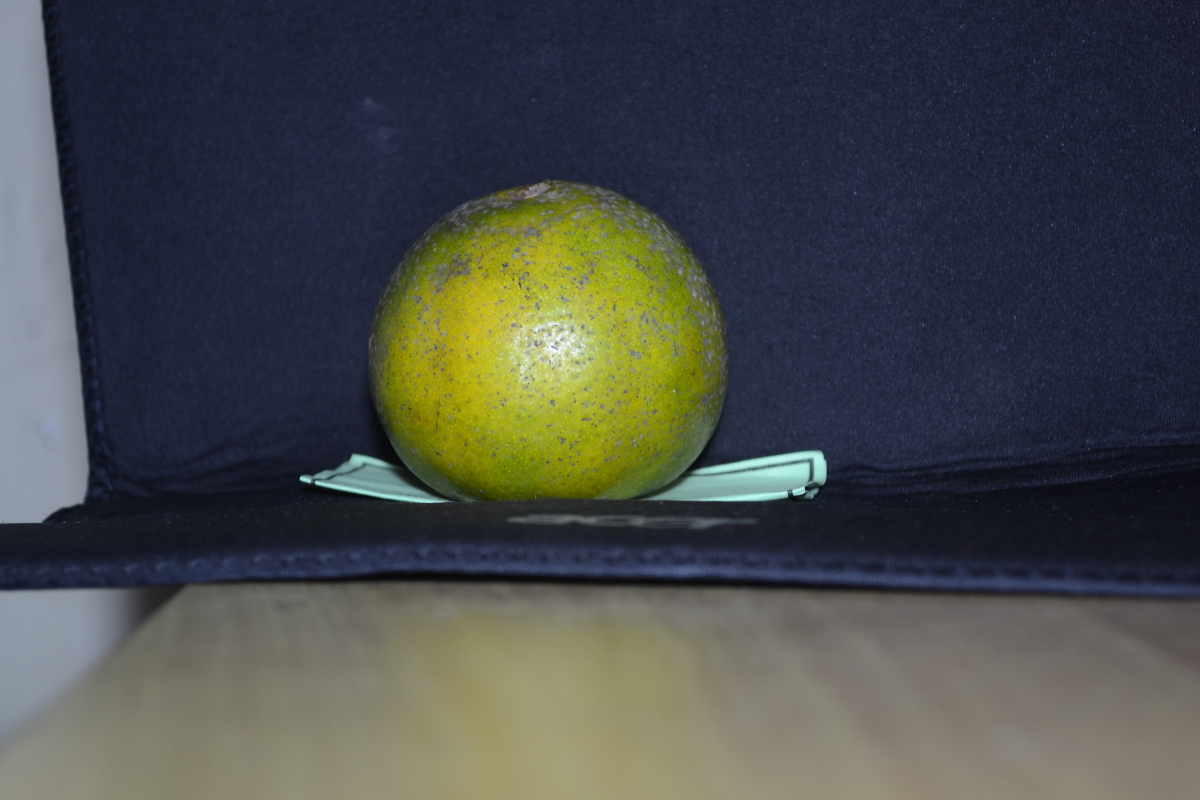
\includegraphics[width=6cm]{tex/3005ori.jpg}

\vskip 1cm
\includegraphics[width=4cm]{../data/DSC_3005.JPG} \qquad
\includegraphics[width=4cm]{../olahdata/proc/smoothcrop/DSC_3005.png}
\caption{Foto asli, foto hasil \emph{crop} dan \emph{resize}, foto yang sudah dibersihkan}
\end{figure}

\subsubsection{\emph{Thresholding}}

Citra dipisahkan ke dalam tiap komponen warna RGB. Untuk tiap komponen warna dihitung nilai \emph{threshold} dengan metode Otsu. Nilai \emph{threshold} ini digunakan pada proses klasifikasi awal \emph{pixel}.


\subsubsection{Klasifikasi \emph{Pixel} Awal}

Pada citra jeruk dilakukan klasifikasi \emph{pixel} awal berdasarkan perbandingan nilai komponen warna \emph{pixel} dengan hasil \emph{threshold} sesuai rumus \ref{classcol}. Hasil yang didapatkan disimpan sebagai matriks angka integer yang menunjukkan kelas-kelas untuk tiap pixel. Tabel \ref{table:preclass3} menunjukkan contoh hasil klasifikasi awal. Gambar \ref{fig:preclassex} adalah visualisasi contoh hasil klasifikiasi awal untuk citra jeruk.

\begin{table}[h]
\centering
\begin{tabular}{|l|l|l|l|l|l|}
\cline{1-6}
\multirow{2}{*}{} & \multirow{2}{*}{Data} & \multicolumn{3}{l|}{\emph{Threshold}} & \multirow{2}{*}{Kelas} \\
\cline{3-5}
 & & $R=82$ & $G=79$ & $B=44$ & \\
\cline{1-6}
1 & $R=50, G=50, B=45$ & 0 & 0 & 1 & 2 \\
2 & $R=10, G=11, B=2$ & 0 & 0 & 0 & 1 \\
3 & $R=120, G=115, B=90$ & 1 & 1 & 1 & 7 \\
\cline{1-6}
\end{tabular}
\caption{Contoh klasifikasi awal \emph{pixel}}
\label{table:preclass3}
\end{table}

\begin{figure}[h]
\centering
\includegraphics[width=4cm]{../olahdata/proc/smoothcrop/DSC_3005.png} \qquad
\includegraphics[width=4cm]{../olahdata/proc/data/seg12a.png}
\caption{Contoh hasil klasifikasi awal untuk citra jeruk}
\label{fig:preclassex}
\end{figure}

\subsubsection{Perhitungan Rata-Rata Intensitas Kelas dan Jarak Antarkelas}

Rata-rata intensitas kelas dihitung dari nilai komponen warna dari semua \emph{pixel} yang masuk ke dalam kelas tersebut, dinyatakan dalam rumus \ref{classavgeq}. Nilai rata-rata tersebut digunakan untuk menghitung jarak antarkelas sesuai rumus \ref{classavgdist}.

\subsubsection{Pembuatan Kelas Baru}

Berdasarkan jarak antarkelas dapat ditemukan kelas-kelas yang bertetangga. Dua buah kelas bertetangga jika keduanya merupakan kelas terdekat bagi kelas lainnya.

\subsubsection{Klasifikasi \emph{Pixel} Akhir}

Untuk setiap kelas baru yang dihasilkan dicari nilai rata-rata intensitas yang baru. Nilai rata-rata intensitas ini merupakan titik-titik pusat kelas.

\emph{Pixel} foto diklasifikasikan ke dalam kelas dengan jarak pusat terdekat. Hasil yang didapat dari langkah ini adalah matriks integer yang berisi kelas-kelas setiap \emph{pixel}.

\subsubsection{Pembuatan \emph{Mask}}

Dari matriks kelas pixel titik-titik \emph{thresholding} untuk mengambil \emph{pixel} yang diklasifikasikan ke kelas tertinggi. Langkah ini menghasilkan citra biner $T$, nilai 1 menunjukkan tekstur normal di bagian tengah jeruk. Lubang-lubang pada citra biner merupakan titik-titik yang digolongkan sebagai cacat. Gambar \ref{fig:highmask} merupakan contoh input dan output proses \emph{threshold}.

\begin{figure}[h]
\centering
\includegraphics[width=4cm]{../olahdata/proc/data/seg12b.png} \qquad
\includegraphics[width=4cm]{../olahdata/proc/data/mask12normal.png}
\caption{Contoh operasi \emph{thresholding} untuk mendapatkan lapisan kelas tertinggi.}
\label{fig:highmask}
\end{figure}

Untuk mendapatkan daerah cacat, dibuat sebuah \emph{mask} $T'$ dengan cara menambal lubang pada citra biner dengan algoritma \emph{hole filling}. Daerah cacat didapatkan dari selisih antara \emph{mask} $T'$ dan citra biner $T$. Langkah ini tidak mendeteksi cacat pada keseluruhan sisi jeruk yang ditampilkan pada citra, bagian tepi jeruk dengan intensitas cahaya lebih rendah dihapus dari $T$. Gambar \ref{fig:holemask} menunjukkan contoh operasi pengisian lubang dan hasil deteksi.

\begin{figure}[h]
\centering
\includegraphics[width=4cm]{../olahdata/proc/data/mask12filled.png} \qquad
\includegraphics[width=4cm]{../olahdata/proc/data/mask12blemish.png}
\caption{Contoh operasi \emph{hole filling} diikuti dengan pencarian cacat dari selisih dengan \emph{mask} daerah normal.}
\label{fig:holemask}
\end{figure}

\subsubsection{Penghitungan Luas Daerah Cacat}

Luas daerah cacat dapat diperkirakan dari prosentase jumlah pixel cacat yang terdeteksi terhadap jumlah pixel \emph{mask} hasil operasi penutupan lubang. Kualitas jeruk dapat ditentukan berdasarkan prosentase cacat sesuai dengan standard SNI. Namun, untuk mendapatkan hasil perhitungan yang akurat objek perlu diputar untuk mendapatkan hasil deteksi pada daerah-daerah yang tidak ikut diproses.

\subsubsection{Perhitungan Akurasi Hasil Deteksi}

Hasil deteksi cacat dengan pengolahan citra dibandingkan dengan citra biner deteksi cacat secara manual yang dibuat dengan perangkat lunak penyunting citra. Ukuran \emph{true positive}, \emph{false positive}, \emph{true negative}, \emph{false negative} diperoleh dari operasi logika terhadap citra biner hasil deteksi pemrosesan, hasil deteksi manual dan \emph{mask} daerah normal yang telah diisi lubangnya. Selanjutnya nilai-nilai tersebut diolah untuk mendapatkan presisi, akurasi dan \emph{recall}.

\end{document}
